% !TeX spellcheck = cs_CZ
{\tikzset{external/prefix={tikz/FYZII/}}
 \tikzset{external/figure name/.add={ch34_}{}}
%---------------------------------------------------------------------------------------------------
% file fey2ch34.tex
%---------------------------------------------------------------------------------------------------
%=========================== Kapitola Magnetizmus látek ============================================
\chapter{Magnetizmus látek}\label{fyz:IIchapXXXIV}
\minitoc
  \section{Diamagnetizmus a paramagnetizmus}\label{fyz:IIchapXXXIVsecI}
  \section{Magnetické momenty a moment hybnosti}\label{fyz:IIchapXXXIVsecII}
  \section{Precese atomových magnetů}\label{fyz:IIchapXXXIVsecIII}
  \section{Diamagnetizmus}\label{fyz:IIchapXXXIVsecIV}
  \section{Larmorova věta}\label{fyz:IIchapXXXIVsecV}
  \section{Klasická fyzika nevysvětluje diamagnetizmus ani 
  paramagnetizmus}\label{fyz:IIchapXXXIVsecVI}
  \section{Moment hybnosti v kvantové mechanice}\label{fyz:IIchapXXXIVsecVII}
  \section{Magnetická energie atomů}\label{fyz:IIchapXXXIVsecVIII}
  \section{Příklady a cvičení}\label{fyz:IIchapXXXIVsecIX}

    \begin{figure}[ht!] %\ref{fyz_fig854}
      \centering
      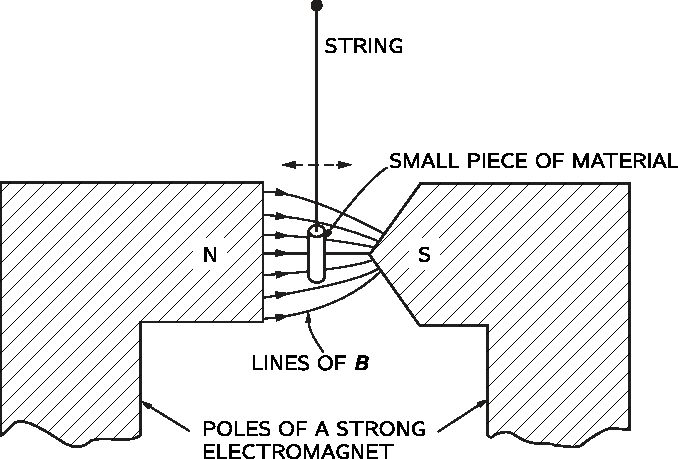
\includegraphics[width=0.7\linewidth]{fyz_fig854.pdf}
      \caption{
               (\cite[s.~707]{Feynman02})}
      \label{fyz_fig854}
    \end{figure}

    \begin{figure}[ht!] %\ref{fyz_fig855}
      \centering
      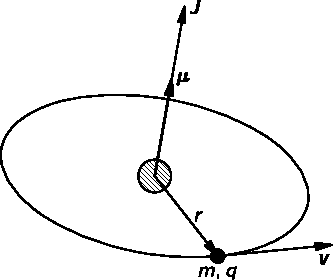
\includegraphics[width=0.7\linewidth]{fyz_fig855.pdf}
      \caption{
               (\cite[s.~707]{Feynman02})}
      \label{fyz_fig855}
    \end{figure}

    \begin{figure}[ht!] %\ref{fyz_fig856}
      \centering
      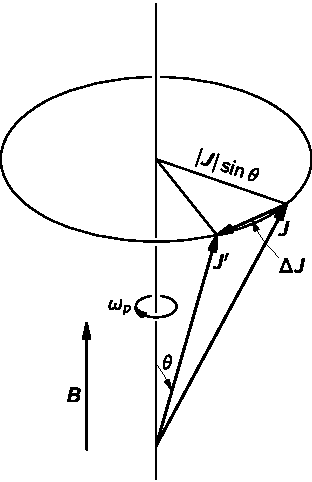
\includegraphics[width=0.7\linewidth]{fyz_fig856.pdf}
      \caption{
               (\cite[s.~707]{Feynman02})}
      \label{fyz_fig856}
    \end{figure}

    \begin{figure}[ht!] %\ref{fyz_fig857}
      \centering
      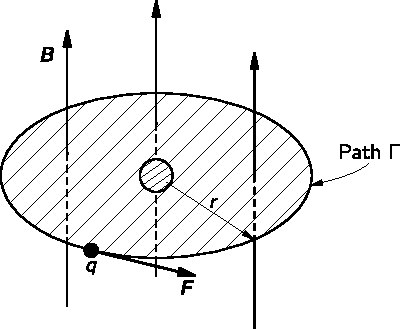
\includegraphics[width=0.7\linewidth]{fyz_fig857.pdf}
      \caption{
               (\cite[s.~707]{Feynman02})}
      \label{fyz_fig857}
    \end{figure}

    \begin{figure}[ht!] %\ref{fyz_fig858}
      \centering
      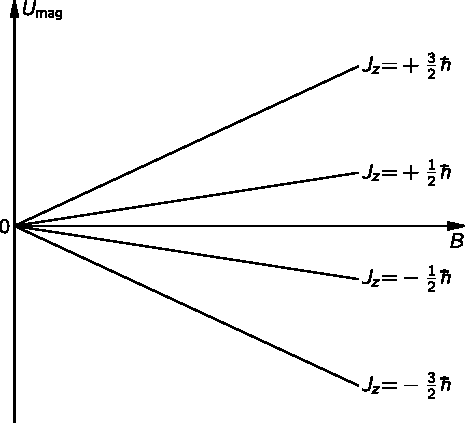
\includegraphics[width=0.7\linewidth]{fyz_fig858.pdf}
      \caption{
               (\cite[s.~707]{Feynman02})}
      \label{fyz_fig858}
    \end{figure}

    \begin{figure}[ht!] %\ref{fyz_fig859}
      \centering
      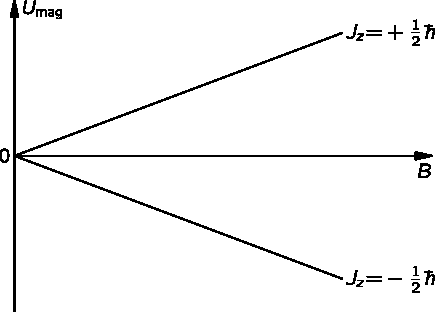
\includegraphics[width=0.7\linewidth]{fyz_fig859.pdf}
      \caption{
               (\cite[s.~707]{Feynman02})}
      \label{fyz_fig859}
    \end{figure}










} %tikzset
%---------------------------------------------------------------------------------------------------
\printbibliography[title={Seznam literatury},heading=subbibliography]
\addcontentsline{toc}{section}{Seznam literatury}